%Bildschirmteilungskallibrierung: 16:9                                                                    |
\documentclass[10pt,aps,prb,twocolumn, nofootinbib]{revtex4-2}

\usepackage{mathptmx}   
\usepackage[T1]{fontenc}

\usepackage[mathscr]{euscript}
    
\usepackage{physics}
\usepackage{amssymb,amsmath}
\usepackage{subfig}
\usepackage{graphicx} 
\usepackage{color}
\usepackage{hyperref}
\usepackage{listings}
\usepackage{blindtext}

\usepackage{tabularx}

\usepackage[a4paper, left=2cm, top=2cm, bottom=2cm, right=2cm]{geometry}

\graphicspath{{./images/}}
%\usepackage[style=phys]{biblatex}
%\bibliography{bibliography.bib} 

% Auskommentieren um Seitenzahl zu entsorgen!
%\pagenumbering{gobble}
\begin{document}
%\addbibresource{bibliography.bib}

\newcommand{\curlybraces}[1]{\left\{#1\right\}}

\title{Das Deutsch-Jozsa-Problem - Lösung mit Quantencomputern}
\author{Florian Klotz}
\noaffiliation
%\affiliation{JGW Sch\"ulerakademie, Papenburg, August 2022}

\begin{abstract}
Das Deutsch-Jozsa-Problem ist eines der ältesten Probleme, mit dem bewiesen werden konnte, das
Quantencomputer einige Probleme schneller als klassische Computer lösen können. Im Folgen soll das
Deutsch-Jozsa-Problem erläutert, und als quantenmechanischer Algorithmus gelöst werden.

\end{abstract}

\maketitle

\section{Das Deutsch-Jozsa-Problem}

\subsection{Allgemeines}

Das Deutsch-Joza-Problem beschreibt die Frage, ob eine Funktion balanciert oder konstant ist. Gegeben ist
daf\"ur eine unbekannte Funktion
\begin{align*}
    f:\{0,1\}^n\rightarrow \curlybraces{0,1} \,.
\end{align*}
Sie gibt f\"ur jedes Eingabebit einen Wert aus. Dabei steht $n$ f\"ur die Anzahl der Eingangsbits und
$\curlybraces{0,1}$ f\"ur die Werte, die Ein- und Ausgangsbits annehmen k\"onnen, also $0$ und $1$. Zudem
ist zugesichert, dass die Funktion entweder konstant oder balanciert ist. $f$ ist unbekannt, also als
"Black Box" gegeben. Somit kann die Definition nicht zum erschließen des Problems verwendet werden. Zudem
wird sie meißt als "Oracle" bezeichnet.

Zudem gibt es eine Anzahl $N = 2^n$ möglicher bin\"arer Eingaben, die auf die Eingabebits geschrieben
werden und jeden Zustand beschreiben, die die Eingabebits annehmen k\"onnen.
Die Funktion ist konstant, wenn sie für alle Eingangswerte den selben Ausganswert zur\"uckgibt.
Balanciert ist sie, wenn sie f\"ur exakt die H\"alfte der Eingabewerte den einen und f\"ur die andere
H\"alfte den anderen Wert zur\"uckgibt.

\subsection{Geschichte}

Das Deutsch-Jozsa-Problem ist eine Erweiterung des Deutsch-Problems\cite{Deutsch-Jozsa:1}.
Es wurde 1992 durch Richard Jozsa verallgemeinert, nachdem David Deutsch 1985 das nach ihm benannte
Problem aufgestellt hatte.
Dieses besch\"aftigt sich mit dem selben Ansatz wie das Deutsch-Jozsa-Problem, jedoch mit nur einem Bit,
also $n=1$.

Somit ist die Funktion konstant, wenn
\begin{align*}
    f(0)=f(1)\,.
\end{align*}
bzw. balanciert wenn
\begin{align*}
    f(0)\neq f(1)\,.
\end{align*}


\section{L\"osung des Deutsch-Jozsa-Problems}
Das Deutsch-Jozsa-Problem hat zwar grunds\"atzlich keine Realen Anwendungen, außer
Geschwindigkeitssteigerungen durch Quantencomputer zu zeigen, kann aber etwas leichter vorstellbar
gemacht werden. So kann sich die Funktion, die betrachtet wird, als teurer z.B. elektrischer
Komponent oder Chip vorgestellt werden. Ziel ist es den Chip so wenig wie m\"oglich zu benutzen, um die
Abnutzung möglichst gering zu halten.

F\"ur die folgenden L\"osungswege wird die balancierte Funktion
\begin{align*}
    f(x)&=x_0 \oplus x_1 x_2
\end{align*}
verwendet.
Die Funktion hat also drei Eingabebits. Zuerst wird $x_1$, also Bit 1 mit $x_2$, also Bit 2 multipliziert.
Dieses Ergebniss wird dann bin\"ar auf $x_0$, das 0-te Bit addiert.
So ergibt sich folgende Ergebnisstabelle:
\begin{center}
    \begin{tabularx}{0.45\textwidth}{|| >{\centering\arraybackslash}X | >{\centering\arraybackslash}X ||}
        \hline
        Bin\"are Darstellung & Funktion\\
        $x_2 x_1 x_0$ & $f(x)=x_0 \oplus x_1 x_2$\\
        \hline
        000 & 0\\
        001 & 1\\
        010 & 0\\
        011 & 1\\
        100 & 0\\
        101 & 1\\
        110 & 1\\
        111 & 0\\
        \hline
    \end{tabularx}
\end{center}

\subsection{Klassische L\"osung des Deutsch-Jozsa-Problems:}
Klassisch wird das Problem durch einfaches Ausprobieren gel\"ost. Da zugesichert wird, dass die Funktion
nur balanciert oder konstant sein kann, kann die Antwort durch Ausschlussverfahren ermittelt werden.
Falls mehr als die H\"alfte der Eingabewerte den selben Wert haben, muss die Funktion konstant sein,
da f\"ur eine balancierte Funktion nur die H\"alfte der Ausgaben gleich sein d\"urfen.
Unterscheiden sich jedoch mindestens zwei Ausgabewerte voneinander, so muss die Funktion balanciert sein,
da bei einer konstanten Funktion alle Ausgaben gleich sind.

So ergibt sich eine Maximalanzahl an Eingaben, die jedoch regul\"ar ausprobiert werden m\"ussen
\begin{align*}
    N_{max} = \frac{1}{2}N+1 = 2^{n-1} + 1\,.
\end{align*}
Die Maximalanzahl beschreibt zudem auch die Maximale Laufzeit, da f\"ur jede Eingabe die selben
Operatoren angewandt werden.

Bei der gegebenen Funktion $f(x)=x_0 \oplus x_1 x_2$ k\"onnen z.B. die Kombinationen $000$ bis $011$ oder
$100$ bis $111$ ausprobiert werden.

\subsection{L\"osung mit Quantencomputern}
Mithilfe von Quantencomputern kann das Problem wesentlich schneller gel\"ost werden, der ben\"otigte
Algorithmus ist jedoch wesentlich komplizierter.

Zuerst werden die $n+1$ Qubits auf den Basisvektor $\ket{0}$ initialisiert. Das $n+1$te, sog. Ancilla Bit
wird danach invertiert, um den Basisvektor $\ket{1}$ darzustellen. Danach wird auf alle Bits n das sog.
Hadamard-Gate angewandt. Dadurch werden die Qubits in Superpositionen zwischen $\ket{0}$ und $\ket{1}$
gebracht. Die Qubits haben also gleichzeitig den Wert $\ket{0}$ und $\ket{1}$ und nehmen alle m\"oglichen
Eingaben gleichzeitig ein.
Dies wird wie folgt dargestellt:
\begin{align*}
    \hat{\mathscr{H}}\ket{0} &= \frac{1}{\sqrt{2}} \bigl(\ket{0}+\ket{1}\bigr)\\
    &= \frac{1}{\sqrt{2}} \begin{pmatrix}1\\1\end{pmatrix}
    = \ket{+}\,, \\[1ex]
    \hat{\mathscr{H}}\ket{1} &= \frac{1}{\sqrt{2}} \bigl(\ket{0}-\ket{1}\bigr)\\
    &= \frac{1}{\sqrt{2}} \begin{pmatrix}1\\-1\end{pmatrix}
    = \ket{-}\,.
\end{align*}
Als Circuit:
\begin{figure}[h]
    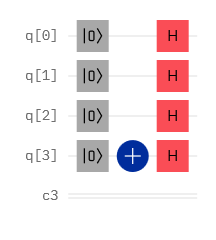
\includegraphics[scale=0.5]{hadamard01}
\end{figure}

Danach werden die resultierenden Eingabebits $\ket{+}$ und das Ancilla Bit $\ket{-}$ in die Abbildung
von $f$ auf die Basisvektoren $\ket{0}$ und $\ket{1}$ gegeben und dort verrechnet. Das Ergebnis der
Eingabe wird auf das Ancilla bit bin\"ar addiert\cite{Deutsch-Jozsa:1}. Dies bildet insgesamt das Oracle
$U_f$ welches auf alle Bits angewandt wird:
\begin{figure}[h]
    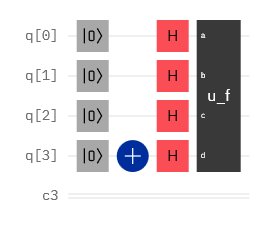
\includegraphics[scale=0.5]{U_f}
\end{figure}

Das Ancilla-Bit, auf dem theoretisch indirekt das Ergebniss steht wird nun weggeworfen, da es nicht
weiter  gebraucht wird. Auf die restlichen Qubits werden wieder Hadamard-Gates angewandt. Danach werden
die drei Eingangsqubits gemessen:
\begin{figure}[h]
    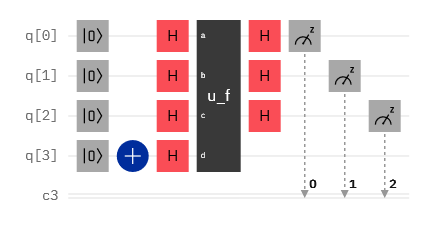
\includegraphics[scale=0.5]{hadamard02}
\end{figure}

Ist die Funktion balanciert, so ist die Wahrscheinlichkeit $\ket{000}$\cite{Deutsch-Jozsa:2}, also auf
jedem Qubit $0$ zu messen gleich $0$. Kann also nie gemessen werden. Ist die Funktion konstant, so ist
die Wahrscheinlichkeit $\ket{000}$ zu messen $1$\cite{Deutsch-Jozsa:2}. Daher wird auf jedem Qubit immer
$0$ gemessen. So kann das Deutsch-Jozsa-Problem mit nur einer einzigen Messung der Funktion gel\"ost
werden.

Leider erschließt sich mir die Funktion des Ancilla-Bits nicht. Bei Quantencomputern müssen alle
Operationen umkehrbar sein. Ancilla-Bits werden z.B. verwendet, wenn dies nicht der Fall 
ist\cite{Ancilla:1}. Weiterhin werden sie verwendet, um Circuits zu vereinfachen usw.\cite{Ancilla:1}.

Tats\"achlich funktioniert der Algorithmus wie oben dargestellt nicht, da mit einer Wahrscheinlichkeit
von ca. $25\%$ $\ket{000}$ gemessen wird.

Ein funktionierender Versuchsaufbau ist:
\begin{figure}[h]
    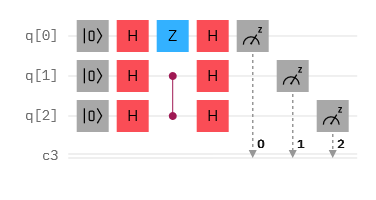
\includegraphics[scale=0.5]{Functioning}
\end{figure}
\\wobei
\begin{figure}[h]
    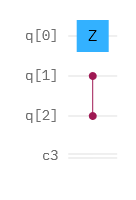
\includegraphics[scale=0.5]{Function}
\end{figure}
\\die Funktion $f(x)=x_0 \oplus x_1 x_2$ darstellt.

Leider habe ich kein genaues Verst\"andniss, wie genau das Ancilla-Bit in eine beliebige Funktion bzw.
in L\"osungen des Deutsch-Jozsa-Problems integriert werden k\"onnte. Zudem hat auch der Kursleiter mit
dem ich in Korrespondenz stand keine zufriedenstellende Antwort gegeben und hat mir zwar eine Rechnung
angeboten, sich jedoch seitdem nichtmehr gemeldet.

Zuk\"unftige \"Anderungen an diesem Dokument k\"onnen ggf. eingesehen werden unter:
\url{https://github.com/DeLumberjack/Schuelerakademie.git}

\newpage
\bibliography{bibliography.bib}
\bibliographystyle{ieeetr}
\end{document}